\documentclass[12pt,twoside]{article}

\usepackage{jmlda}
%\NOREVIEWERNOTES
\title
[Применение методов машинного обучения в задаче улучшения разрешения снимков] % Краткое название; не нужно, если полное название влезает в~колонтитул
{Применение методов машинного обучения в задаче улучшения разрешения снимков, полученных со спутника}
\author
[Автор~И.\,О.] % список авторов для колонтитула; не нужен, если основной список влезает в колонтитул
{Белозерцев~A.\,О., Воскресенский~Н.\,Д., Грибова~О.\,Б., Казаков~A.\,А., Мурзаев~Я.\,А., Хохлов~А.\,А., Шабалина~А.\,А.} % основной список авторов, выводимый в оглавление
[Белозерцев~A.\,О.$^1$, Воскресенский~Н.\,Д.$^1$, Грибова~О.\,Б.$^1$, Казаков~A.\,А.$^1$, Мурзаев~Я.\,А.$^1$, Хохлов~А.\,А.$^1$, Шабалина~А.\,А.$^1$] % список авторов, выводимый в заголовок; не нужен, если он не отличается от основного
\thanks
{ 
	Научный руководитель:  Матвеев~И.\,А. 
	Задачу поставил:  Мурынин~А.\,Б.
	%Консультант:  Консультант~И.\,О.
	}
\email
{author@site.ru}
\organization
{$^1$Московский физико-технический институт (государственный университет)}
\abstract
{Данная работа посвящена исследованию вопроса повышения разрешения мультиспектральных изображений. Рассмотрены разные метрики оценки качества улучшения пространственного разрешения изображений, показана энтропия изображения как идентификатор потерь информации и ее корреляция с преобразованием над изображением. Предложены подход для анализа изображений, алгоритм повышения разрешения путем использования опорных изображений, метод оптимизации параметров данного алгоритма. Проведен сравнительный анализ с аналогичными подходами. Найдены условия максимизации энтропии восстановленного изображения.
	
	\bigskip
	\textbf{Ключевые слова}: \emph {ключевое слово, ключевое слово,
		еще ключевые слова, еще еще ключевое слово}.}
\titleEng
{Entropy maximization in an image various types of transformations}
\authorEng
{Belozertsev~A.\,O.$^1$, Voskresenskiy~N.\,D.$^1$, Gribova~O.\,B.$^1$, Kazakov~A.\,A.$^1$, Murzaev~Y.\,A.$^1$, Khokhlov~A.\,A.$^1$, Shabalina~A.\,A.$^1$}
\organizationEng
{$^1$Moscow Institute of Physics and Technology (State University)}
\abstractEng
{English abstract.
	
	\bigskip
	\textbf{Keywords}: \emph{keyword, keyword, more keywords, moooooore keywords}.}
\newcommand\labelfig{Рис.}
%\graphicspath{{/pics/}}

\begin{document}
\maketitle
%\linenumbers
\section{Введение}
	Основной целью данной работы является разработка алгоритма повышения пространственного разрешения мультиспектральных изображений и изображений с узким диапазоном частот. 
	
	Предметом исследования являются изображения с различным набором частот, имеющие низкое пространственное разрешение, а также панхроматические и RGB-изображения.
	
	В настоящее время аэрокосмическая съемка является основным инструментом для исследований в таких областях как георазведка, метеопрогнозирование, картография, экологический мониторинг и др. При работе со снимками поверхности земли наиболее острой является проблема низкого разрешения полученных трехканальных (RGB) и узкоспектральных изображений, влекущая за собой потерю информативности. Решению задачи повышения качества снимков и посвящена данная работа.
	
	Потребность в получении снимков высокого качества возникает при анализе изображений для распознавания объектов \cite{visilter2009rus}, при мониторинге территорий на основе аэрокосмических данных в аграрной \cite{murynin2013} и нефтегазовой \cite{bondur2012aero} отраслях, для регистрации и прогнозирования морского волнения \cite{bondur2016rusvosstanovlenie,bondur2016rusoptimalniy}. Кроме того, повышение разрешения снимка может использоваться для  повышения точности навигации летательных аппаратов \cite{ishutin2016rus,visilter2016ruscomplexirovaniye}.
	
	Для решения задачи улучшения качества снимков поверхности земли предлагается использовать методы машинного обучения, в частности нейронные сети. 
	
	В работе \cite{gorokhovskiy2017rus} изложен вероятностный алгоритм повышения разрешения мультиспектрального изображения при помощи опорного снимка в виде панхроматического изображения более высокого качества. В \cite{gurchenkov2016rus,bochkareva2016rus} предложены методы улучшения качества, построенные на экстраполяции или объединении пространственных спектров.
	
	Одним из основных преимуществ представленного решения является использование универсального метода - нейронной сети, который позволяет достичь высоких результатов. Однако, данный алгоритм имеет ряд недостатков, среди которых можно отметить отсутствие его физической интерпретации, а также необходимость наличия больших вычислительных мощностей для реализации.
	
	Целью представленного эксперимента является создание модели нейронной сети, которая смогла бы увеличить пространственное разрешение лучше имеющихся на данный момент аналогов, основанных на аналитических подходах. В качестве данных использовались снимки с космических спутников.

	В работе \cite{schuler2013machine} предлагается метод, представляющий собой восстановление изображения с помощью последовательного применения Direct deconvolution и MLPs («Multi layer perceptrons»).

	В статье \cite{burger2012image} метод MLPs сравнивается с методом BM3D. Сравнение показывает приблизительно одинаковые результаты (PSNR ~ 30dB). 

	В работе \cite{dong2016image} применяется метод, который состоит в последовательном применении трех конволюций с разными параметрами. Эксперимент проведен как с тремя каналами (RGB), так и с одним. Данная работа на момент 2015-2016 года является лучшей по двум параметрам: скорость и качество. В качестве метрики сравнения берется PSNR - пиковое отношение сигнал/шум. 
	
	В работе \cite{johnson2016perceptual} используется сравнивается две различных функции потерь, одна из которых уже упомянутая выше PSNR, а вторая использует один из слоев сверточной сети. Для работы последнего способа используется предобученная сеть VGG-16, что дает выигрыш в скорости, так как нет надобности в ее обучении на каждой итерации.

	
\section{Обозначения}
	Введем следующие обозначения:
	\begin{itemize}
		\item $x$ -- исходное изображение
		\item $y$ -- изображение с пониженным разрешением, полученное некоторым преобразованием из $x$. $y$ подается на вход алгоритма.
		\item $z$ -- изображение c повышенным разрешением на выходе алгоритма
		\item $x(i,j)$ -- пиксель под номером $(i,j)$ изображения $x$ 
		\item $MAX_x$ -- пиксель максимальной яркости в изображении $x$
	\end{itemize}
	
\section{Постановка задачи}
	Пусть дано некоторое изображение плохого качества (с недостаточным разрешением). Необходимо представить метод увеличения разрешения изображения $y$ (размера $m\times n$), результат которого превосходит результаты методов, представленных в литературе. В качестве метрики качества работы алгоритма выберем PSNR для удобства сравнения с существующими методами. 
	\begin{gather}
		PSNR = 10\lg\bigg(\frac{MAX_x^2}{MSE} \bigg),
	\end{gather}
	где
	\begin{gather}
		MSE = \frac{1}{mn}\sum_{i=0}^{m-1}\sum_{j=0}^{n-1}\big[x(i,j)-z(i,j)\big]^2
	\end{gather}
	
\section{Описание алгоритма}

	В данной работе рассматривались два подхода к решению задачи восстановления изображения. 

	На начальном этапе моделирования использовалась линейная нейронная сеть, состоящая из девяти слоев. Для обучения были использованы изображения размера $30 \times 30$ пикселей в общем количестве около 2700 образцов, полученные разделением изображени $1560 \times 1560$. Ухудшение изображения проводилось усреднением областей $3 \times 3$, итоговое изображение имело размер $10 \times 10$ пикселей.
	
	Ухудшенное изображение подавалось на вход сети. После каждого линейного слоя размер изображения увеличивался на 100 пикселей. В качестве нелинейной функции активации между каждым слоем использовалась ReLu. Она равна нулю, если на вход ей подается отрицательное значение, следовательно, все выходы последнего слоя, имеющие отрицательное значение, на итоговой картинке будут выглядеть как битые пиксели. С целью решения данной проблемы на в конце выполнялось увеличение размера изображения с 900 до 3600 пикселей с целью проведения последующего усреднения. Результаты обработки представлены на рисунке 1.




\begin{figure}[h]
	\centering
	\subfloat[оригинал -- x]{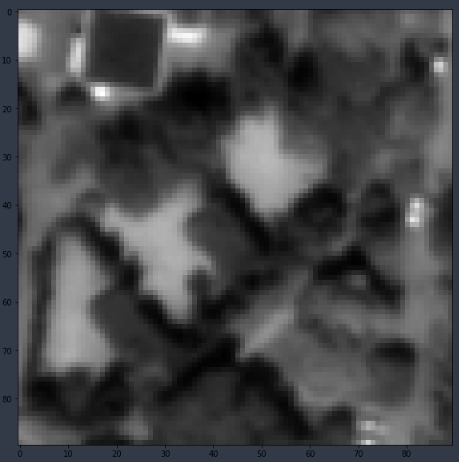
\includegraphics[width=0.3\textwidth]{x.jpg}}
	\subfloat[пониженное разрешение -- y]{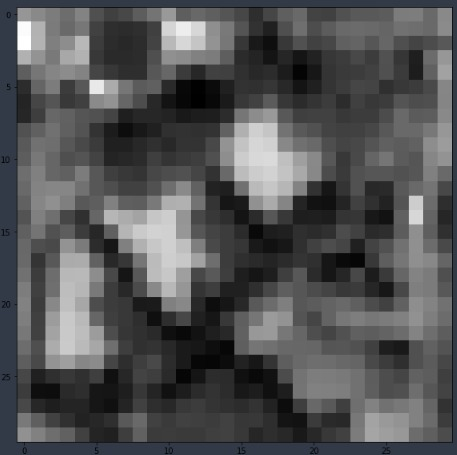
\includegraphics[width=0.3\textwidth]{y1.jpg}}
	\subfloat[результат -- z]{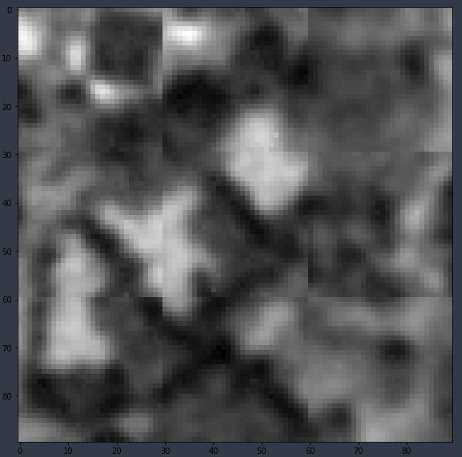
\includegraphics[width=0.3\textwidth]{z_linear.jpg}}\\
	\caption{Линейная нейронная сеть}
	\label{fig:linear}
\end{figure}



	На восстановленном изображении видны швы, их наличие связано с независимостью исходных изображений друг от друга. Кроме того, данная сетка обладает высоким риском переобучения из-за большого числа параметров сети, в сравнении с объемом данных. В связи с этим было решено прекратить разработку данного алгоритма.
	
	На втором этапе моделирования мы пересмотрели принцип формирования набора исходных данных и для создания обучающей выборки были взяты области $9 \times 9$ пикселей, из которой, путем усреднения областей $3 \times 3$, получалась матрица $3 \times 3$.  После данной процедуры производился сдвиг на 3 пикселя, и процедура повторялась. В основе данного решения лежит идея того, что на значение пикселя влияют лишь его близлежащие соседи, которые могут содержать в себе информацию о том же объекте, что и в целевом пикселе. Поэтому наиболее значимой для восстановления одного пикселя, полученного усреднением квадрата $3 \times 3$ пикселей, является область $4 \times 4$. Однако, граничные пиксели являются элементами соседних квадратов $3 \times 3$, которые так же подверглись усреднению, что вынуждает брать для обучения всю область $9 \times 9$ или что тоже самое $3 \times 3$ в усредненном формате.
	
	Для ухудшенного изображения $3 \times 3$ производилась билинейная интерполяция с целью увеличения размера изображения до размера $9 \times 9$. После чего интерполированное изображение подвергается процедуре восстановления изображения. Она состоит из применения 9 различных конволюций к центральной области $4 \times 4$. Каждая конволюция имеет ядро размером $3 \times 3$, обучение которого происходит независимо от остальных. Итого, необходимо подобрать 81 параметр, тогда как общее количество образцов в одной картинки порядка 270 000. Таким образом мы устраняем риск переобучиться. Результат применения данного алгоритма показан на рисунке 2.

\begin{figure}[h]
	\centering
	\subfloat[оригинал -- x]{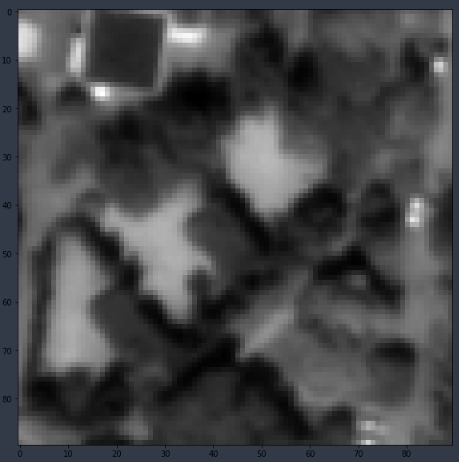
\includegraphics[width=0.3\textwidth]{x.jpg}}
	\subfloat[пониженное разрешение -- y]{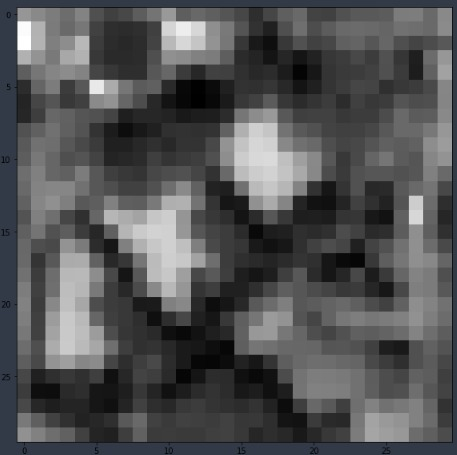
\includegraphics[width=0.3\textwidth]{y1.jpg}}
	\subfloat[результат -- z]{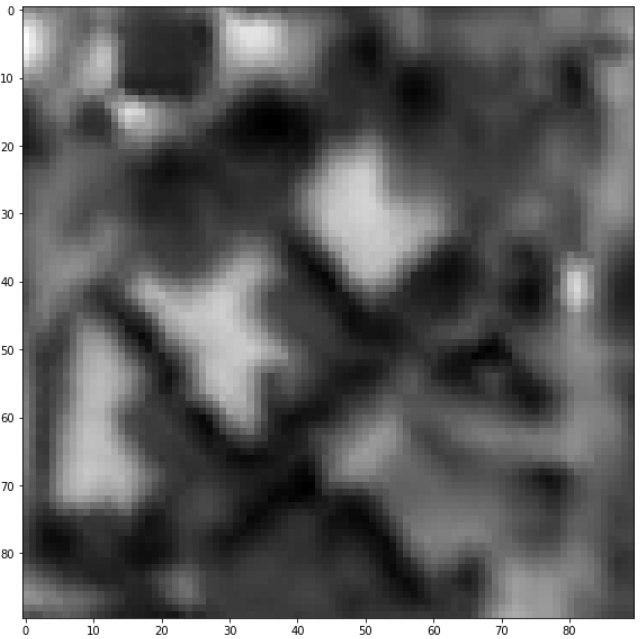
\includegraphics[width=0.3\textwidth]{z_9_conv.jpg}}\\
	\caption{Использование девяти независимых конволюций}
	\label{fig:9conv}
\end{figure}


	
\section{Вывод}

	Подводя итоги можно добавить, что результаты, полученые последней моделью, были сравнены с результатом билинейной интерполяцией. Аналогичное сравнение альтернативных методов восстановления изображений было приведено в работах \cite{dong2016image, johnson2016perceptual}. В качестве метрики использовали MSE, так как в большинстве статей \cite{schuler2013machine, burger2012image, johnson2016perceptual} утверждается наличие обратнопропорциональной зависимости от PSNR. Данное сравнение показало уменьшение значения MSE в 3 раза относительно билинейной интерполяции. Это, а также и визуальная оценка полученных изображений позволяет утверждать о положительном результате описанного способа улучшения качества изображения.

\bibliographystyle{unsrt} %unsrt - for sorted bibliography / plain - for unsertoed bibliography
\bibliography{Project24}

% Решение Программного Комитета:
%\ACCEPTNOTE
%\AMENDNOTE
%\REJECTNOTE
\end{document}
